\documentclass[12pt]{article}

\title{ECE4063 - Image Thresholding}
%\subtitle{Progress Report}
\author{Emmanuel Jacyna - 24227498 \and James Anastasiou - 23438940}
\date{\today}

\usepackage[T1]{fontenc}
\usepackage[utf8]{inputenc}
\usepackage{rotating}
\usepackage{subfig}

\usepackage{graphicx}
\usepackage{tabularx}
\usepackage{float}
\usepackage{amsmath}
\usepackage{listings}
\bibliographystyle{unsrt}


\begin{document}
\pagestyle{myheadings}
  \maketitle
  \pagebreak
  \tableofcontents
  \pagebreak
  \section{Introduction}
  This document represents our findings for Assignment 2 of ECE4063. It is organised into three major sections, assumptions, solution documentation, and a discussion of potential improvements to the project.\\
  
  The task at hand is to perform binary thresholding on an image for use in a bionic eye. The target platform is an Altera Cyclone II FPGA. In order to threshold the image, a histogram of the pixel greyscale values is calculated and used to find the 50th percentile grey scale value. This value is then used to decide whether to colour pixels white or black, performing a total threshold.
  
  \section{Assumptions}
  When thresholding images, we assume that an image where 99.9\% of pixels are one value is meaningless to threshold. In the case of the Altera DE2 board with Terasic camera module, the small variation in value is likely to be because of pixel noise. We also believe that as the target is a human vision system, 100\% accuracy is not necessarily the goal, as we prefer an image that makes sense to the human eye. This design decision allowed for a simplification of the logic circuit required to determine the most accurate thresholding value. 
  
  We also assumed that Model Sim testbenches are 100\% completely accurate representations of reality. This assumption was routinely called into question, however after fixing a number of other assumptions, this sole assumption was found to be a valid assumption.
  
 
  \section{Documentation - Basic Requirements}
  \subsection{RGB to Grayscale conversion}
  There are a number of ways to convert 12bit RGB values into 8Bit Grayscale values, these include taking the average between all 3 colour channels, desaturating the channels or performing a weighted average based on the NTSC standard. Each of these approaches has benefits and weaknesses, our design decision was to approximate the NTSC standard weighted average via fixed shift additions. The decision to approximate the results meant the design did not need to include a multiplier or divider circuit, which significantly improved the potential performance. 3 multipliers were replaced with 6 additions, which if optimised appropriately could utilise Carry Save Adder hardware to improve the performance. Unfortunately as a result of approximating the NTSC values, the actual grayscale values produced to not match exactly with the theoretical values, this was found to be incorrect by a maximum of 6 units, which we determined to be not a significant loss in precision compared to the speedup and simplification of hardware seen.

  \subsection{Total Histogram}
  The Total Histogram is the overall module responsible for managing the histogram generation, cumulative histogram generation, histogram storage and retrieval. This module is implemented as two-tiered state machine, providing states and certain substates to handle particular edge cases that arose during testing. This module responds to changes of frame valid and data valid signals to determine whether to calculate the histogram or total histogram, or provide direct read through capabilities.

  \subsubsection{Histogram Module}
  The histogram module provides a wrapper around a single port ram with read while write capabilities. The module is implemented via simple pipelining to minimise the latency of the circuit. The module uses a 20bit wide RAM with 256 addresses in order to calculate the Histogram. The actual operation of the module is rather simple, with only a single edge case to handle, which is introduced by the registering of the output from the ram. This potentially introduces a race condition where an old value is read from the ram before the new value has been written, this is overcome by checking for this condition, and incrementing the registered value by 1 before writing again, as well as holding the registered value and checking if the same situation occurs again. By solving this race condition the histogram always produces the correct number of values.

  Additionally the histogram module also handles clearing it's internal ram, which simplifies the interface for connection to the cumulative histogram module.
  
  \subsubsection{Histogram Module Testbench Results}
  
  \subsubsection{Histogram Module Signal Tap Results}
    \begin{figure}[H]
    \centering{\includegraphics[scale=\textwidth]{Images/Normal\ Histogram.png}}
    \caption{Normal Operation Signal Tap}
    \label{fig:histogram_signal_tap_normal_operation}
  \end{figure}
   \begin{figure}[H]
    \centering{\includegraphics[scale=\textwidth]{Images/Edge\ Case\ Histogram.png}}
    \caption{Edge Case Histogram Signal Tap}
    \label{fig:histogram_signal_tap_edge_case_operation}
  \end{figure}
  \subsubsection{Cumulative Histogram Module}
  The cumulative histogram is significantly more complex than the histogram module, as it is responsible for a number of \textit{administrative} or \textit{house keeping} tasks. The cumulative histogram iterates over the entire contents of the Histogram ram, cumulating the output and storing the result into another RAM for reading by the histogram display modules. Whilst the cumulative histogram module writes the cumulative values, it also stores the normal histogram values into one of two RAM's. This enables the stored RAM to be used for diaply on the next frame whilst the new histogram is being calculated. Once the frame is no longer valid, a toggle is switched so that the correct RAM is overwritten with the new values, and the other RAM is kept for display on the next frame.

  \subsubsection{Cumulative Histogram Testbench Results}

  \subsubsection{Cumulative Histogram Signal Tap Results}
  \begin{figure}[H]
    \centering{\includegraphics[scale=\textwidth]{Images/Normal\ Cumulative.png}}
    \caption{Normal Operation Cumulative Histogram Signal Tap}
    \label{fig:cumulative_histogram_signal_tap_normal_operation}
  \end{figure}

  \subsection{Thresholding Module}
  \subsubsection{Description}
  The thresholding module is very simple. All it needs to do is take in an 8 bit greyscale value and output either a white (255) if the value is above the threshold, or a black (0) if the value is below the threshold. This is accomplished by hooking up a comparator to a multiplexer.
  
  \subsubsection{RTL Diagram}
  \begin{figure}[H]
    \centering{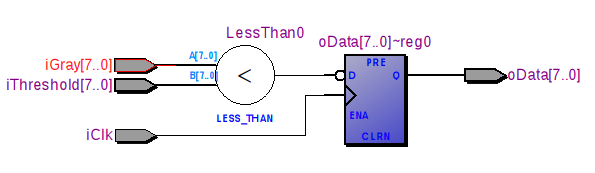
\includegraphics[scale=.8]{Images/ThresholderRTL.png}}
    \caption{Thresholding module RTL}
    \label{fig:thresholder_rtl}
  \end{figure}
  
  
  \subsection{Displaying things}
  \subsubsection{Description}
  In order to display the greyscale image, histogram, cumulative histogram, and thresholded image, we wrote a module to handle multiplexing between them using the switches on the DE2 board, called Arbitrator. This module takes in pixel outputs from the various modules and multiplexes them depending on the switch positions. In order to display images, we simply piggyback on the \(X\_Cont\) and \(Y\_Cont\) signals and modify the \(wr1\_data\) and \(wr2\_data\) inputs to the SDRAM with the appropriate pixel data. \\
      
  Displaying the actual histogram data requires slightly more effort. First we need to extract the histogram data from the histogram RAM and convert the histogram bin contents into pixels for display on the screen. To do this we have a module called HistogramDisplayer. This module takes in the \(Y\_Cont\) signal and uses it to index the histogram RAM. Based on the value obtained from the RAM, it scales the histogram value, and uses the \(X\_Cont\) signal to determine the length of the line to be displayed. 
  \subsubsection{RTL Diagram}
    \begin{figure}[H]
    \begin{center}
        {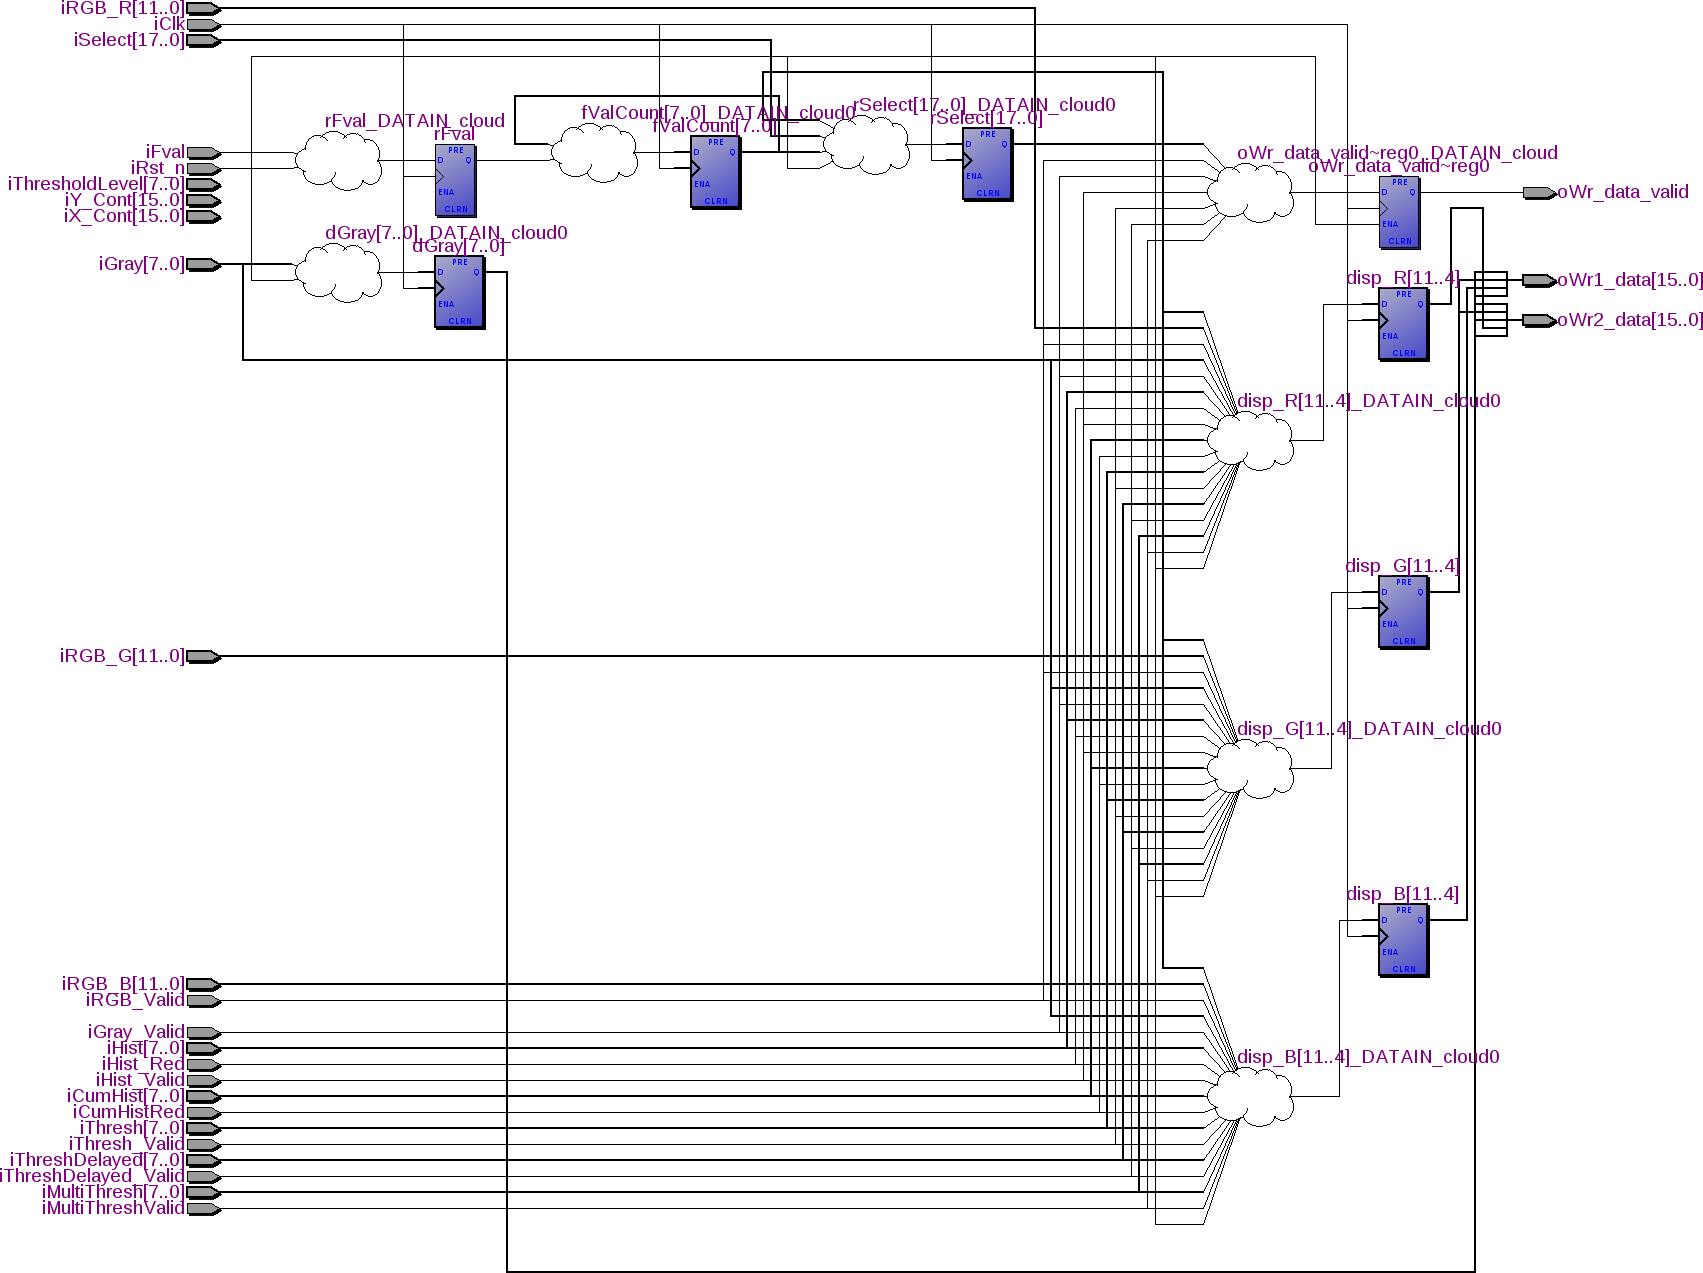
\includegraphics[width=\textwidth]{Images/ArbitratorRTL.png}}
    \end{center}
    \caption{Arbitrator module RTL}
    \label{fig:arbitrator_rtl}
  \end{figure} 
  \subsubsection{RTL Diagram}
    \begin{figure}[H]
    \centering{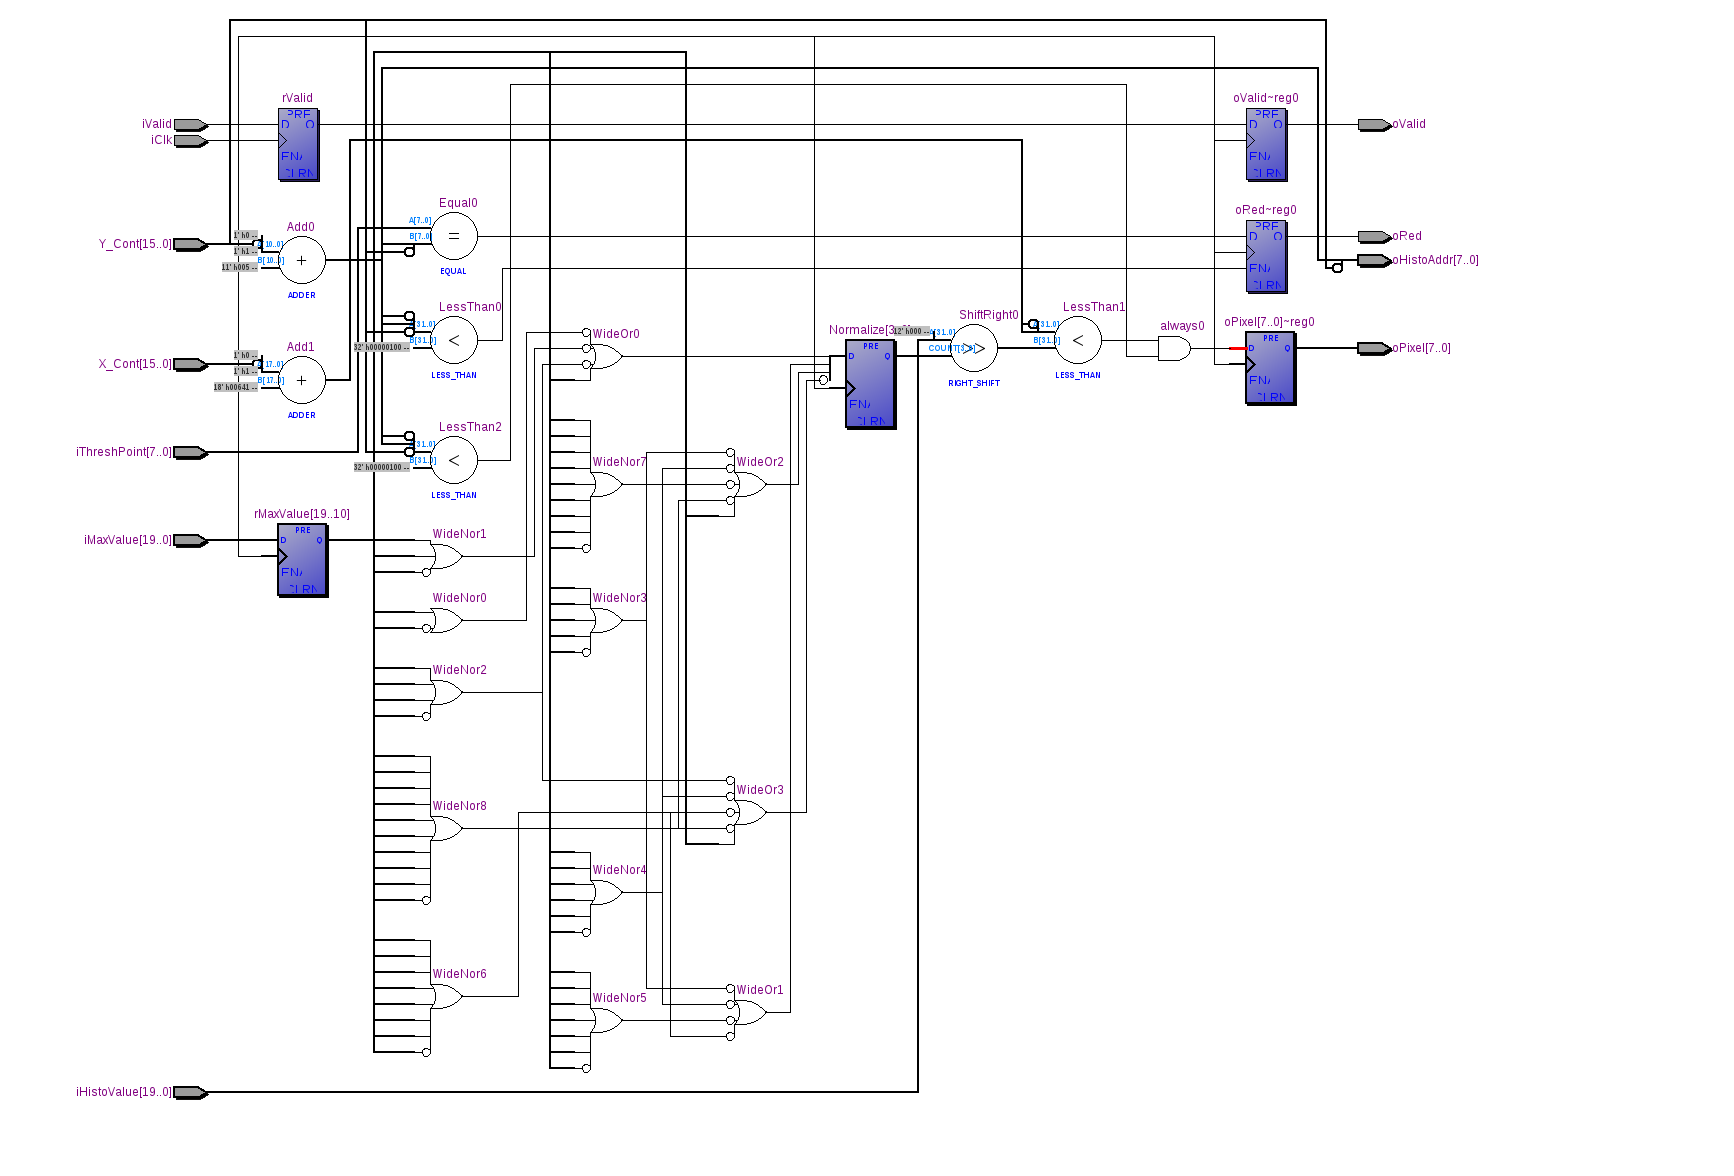
\includegraphics[width=\textwidth]{Images/HistogramDisplayerRTL.png}}
    \caption{HistogramDisplayer module RTL}
    \label{fig:histogram_displayer_rtl}
  \end{figure}
  
  
  \subsection{High Level Overview}
  \begin{figure}[H]
    \centering{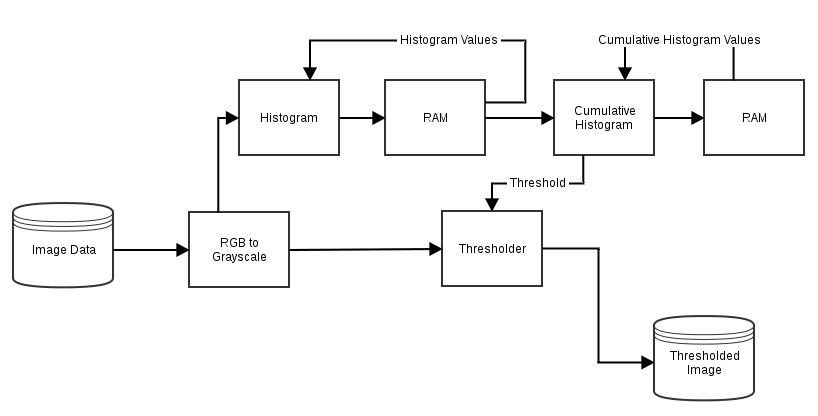
\includegraphics[width=\textwidth]{Images/HistogramOverview.png}}
    \caption{Overview of the image thresholding process}
    \label{fig:histogram_overview}
  \end{figure}
  
  The toplevel module, \texttt{Total\_Module} is fed RGB values from the camera. Those RGB values are then passed through an RGB to Greyscale conversion to output Greyscale values between 0 and 255. These greyscale values are then passed to the histogram module, which uses an internal RAM to count the number of times each greyscale value is encountered. Once the entire image has been processed, the cumulative histogram module is activated. This module uses its own internal RAM to store the cumulative sum of the histogram. Whilst it calculates the cumulative sum, it checks to see when the cumulative sum passes above the 50th percentile (the point when the sum is less than \(800*480/2\)). It saves this point as the threshold value. On the next frame, this value is then passed through to the thresholder module. The thresholder module uses the threshold it has been given to compare incoming greyscale values. Values that are above the threshold are coloured white, and those below are coloured black.
  
  \section{Documentation - Advanced Requirements}
  A summary of how the advanced requirements were achieved
  
  \subsection{Threshold and Display the Correct Frame}
  In order to successfully threshold the frame the theshold was calculated for, we noticed that the \(wr1\_data\) and \(wr2\_data\) wires were not fully packed, and that there was exactly 8 bits of available space that was not utilised. We then recognised that in order to threshold the correct frame, the only information that needs to be delayed that can't be stored on chip was the grayscale values of the image. With this in mind we delayed the gray value and packed the \(wr1\_data\) and \(wr2\_data\) wires with the relevant grayscale values. So the wires are therefore containing data of the form \texttt{16'bXGGG-GGBB-BBBB-BBXX} and \texttt{16'bXGGG-XXRR-RRRR-RRXX} where \texttt{8'bXXXX-XXXX} is the 8 bit grayscale value, split across the 8 available bits of \(wr1\_data\) and \(wr2\_data\).

  On the read side of the SDRAM FIFO, we intercepted the data, unpacked it and ran the resulting grayscale through a thresholder which utilises a stored threshold value generated by the total module. We only enable the display of the threshold interception when the appropriate switch is high, thus providing the delayed outcome.

  \subsection{Divided Threshold}
  In order to divide the display into 2 equal subwindows of half width the \texttt{Y\_Cont} value was used to split the display in half, by a simple comparison with the halfway value of 240, if \texttt{Y\_Cont} was found to be larger than 240, then the larger threshold was used, if it was found to be larger, then the smaller threshold was to be used. This task only required a small alteration to the Cumulative Histogram and Threshold Displayer modules, to account for the increased number of Threshold values to be generated and used.

  \subsection{Smooth Divided Threshold}
  In order to remove the block artifacts generated by the significant step difference between the two thresholds, the middle 128 (or in our final version 256) pixels were thresholded via a linear interpolation between the two thresholds. This was achieved by using fractional bits. In the 128 bit case, the difference between the two thresholds, delta is calculated. This value is 8 bits wide, and as such it is shifted 24 bits to the left, generating a 32 bit integer. This 32 bit value is then shifted right 7 bits, to divide it by 128, this is the step value. This 32bit step value is then subtracted from a synthetic threshold (which is just the larger threshold shifted left 24bits to create another 32bit integer). This subtraction only occurs immediately following \texttt{X\_Cont} begin 799, to ensure that it only occurs once per display column. Using fractional bits allows the full precision of division by 128 to be maintained in the larger synthetic threshold variable, which is right shifted 24 bits to retrieve an 8 bit value describing the actual threshold. This process is used because it prevents a loss of \(carry\) information. In our actual code we used a window of 256 pixels instead of 128, due to the fact that the larger window provided a much nicer effect.

  Our implementation of fractional bits was very inefficient, significant improvements could be found by only shifting left by the absolutely minimum needed amount, the extra bits gained by a shift of 24 instead of 7 (or 8 in our case) provide no extra precision in our use case. The extra bits only serve to slow down that aspect of the circuit, which is a clear example of something that could be easily optimised away.
  
  \section{Acknowledgements}
  
  \section{Improvements}
  
  \section{Conclusion}
  
  \newpage
  \newpage
  \section{Appendix C - Testbench Results}
  \subsection{RGB2GRAY}
    In order to test the \texttt{RGB2GRAY} module, the greyscale conversion, a testbench was written that took as inputs the RGB values of an image, and outputted a file containing the grey values calculated by the modelsim simulation. This was then compared to the MATLAB rgb2gray function results. The mean difference between the MATLAB and Verilog functions was only .56, not enough to visibly affect the image output. This was deemed to be well within tolerable bounds.
\begin{figure}[H]
  \centering
  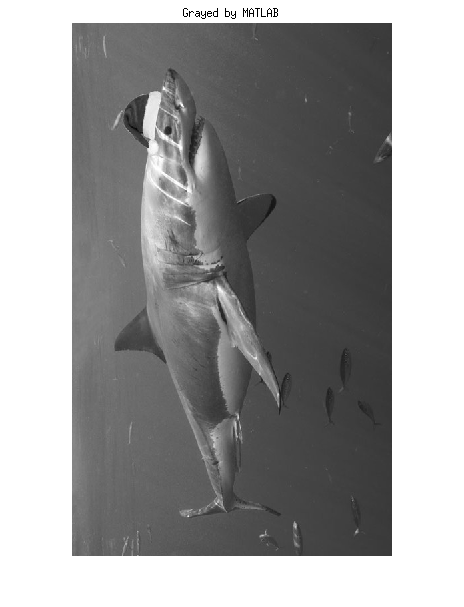
\includegraphics[height=300pt, angle=-90]{Images/RGB2GRAY/MATLAB.png}
  \captionof{figure}{MATLAB rgb2gray result}
\end{figure}
\begin{figure}[H]
  \centering
  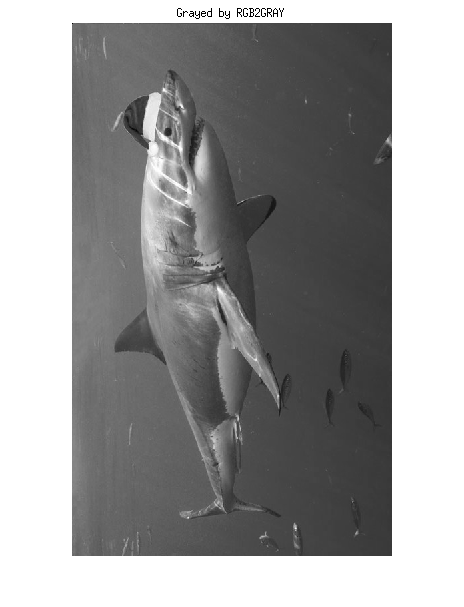
\includegraphics[height=300pt, angle=-90]{Images/RGB2GRAY/Verilog.png}
  \captionof{figure}{RGB2GRAY.v result}
\end{figure}
\begin{figure}[H]
  \centering
  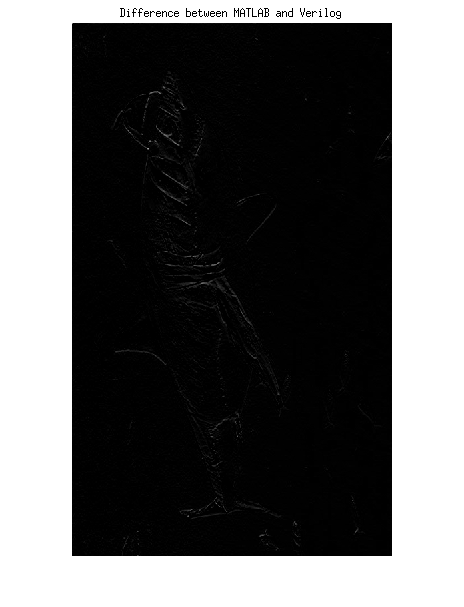
\includegraphics[height=300pt, angle=-90]{Images/RGB2GRAY/Difference.png}
  \captionof{figure}{Difference between the two}
\end{figure}

    
  \newpage
  \subsection{Histogram}
  In order to test the \texttt{Histogram} module, a testbench was written to read in precalculated greyscale values and output a histogram. This histogram was then compared to the histogram generated by matlab. Both histograms are very similar. The mean difference between the two is 3.15.
  \begin{figure}[H]
    \centering{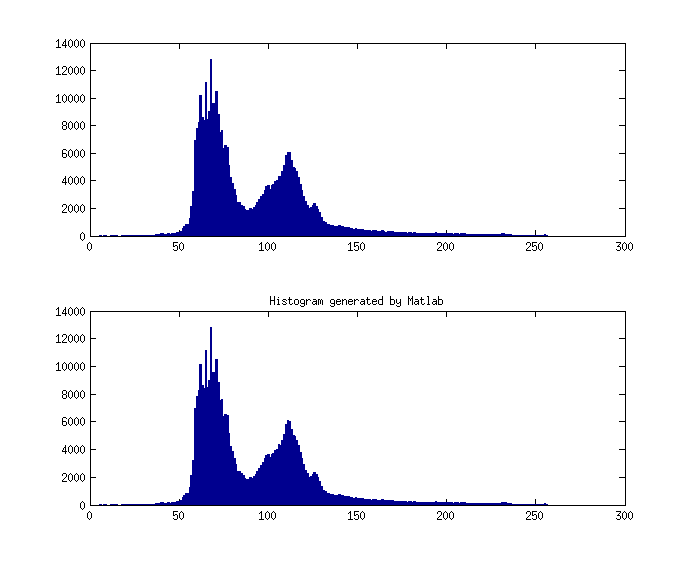
\includegraphics[scale=.8]{Images/HistogramTestbench.png}}
    \caption{Comparison of histogram generated by Histogram module and by matlab}
    \label{fig:histogram_testbench}
  \end{figure} 
  
  \newpage
  \subsection{CumulativeHistogram}d
    In order to test the \texttt{CumulativeHistogram} module, a testbench was written to read in a histogram (generated by \texttt{Histogram} module). The cumulative histogram was then calculated and compared to that generated by matlab. The two cumulative histograms are identical.
  \begin{figure}[H]
    \centering{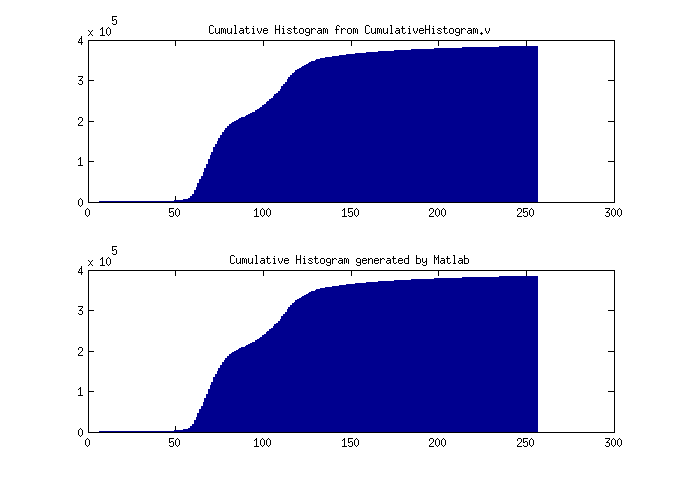
\includegraphics[scale=.8]{Images/CumulativeHistogramTestbench.png}}
    \caption{Comparison of cumulative histogram generated by Cumulative Histogram module and by matlab}
    \label{fig:cumulative_histogram_testbench}
  \end{figure} 
  
  \newpage
  \subsection{Total\_Histogram}
    In order to test the \texttt{Total\_Histogram} module, a testbench was written to read in precalculated greyscale values and output a histogram and a cumulated histogram. The result is the same as those calculated with the separate Histogram and CumulativeHistogram testbenches.
  \begin{figure}[H]
    \centering{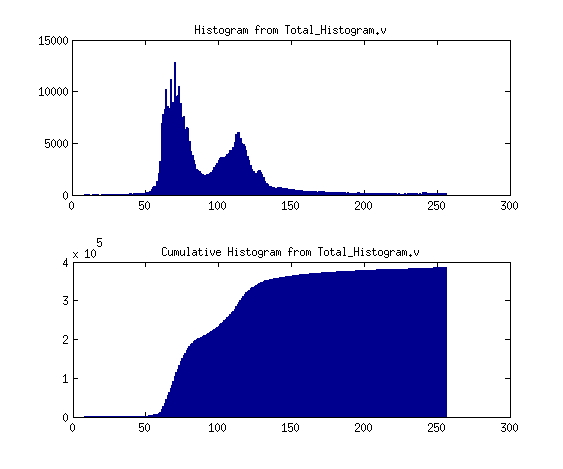
\includegraphics[scale=.8]{Images/Total_HistogramTestbench.png}}
    \caption{Cumulative Histogram and Histogram generated by \texttt{Total\_Histogram} module}
    \label{fig:cumulative_histogram_testbench}
  \end{figure} 
  
  \newpage
  \subsection{HistogramDisplayer}
  In order to test the \texttt{HistogramDisplayer} module, a testbench was written to read in histogram values and output the same image that would be outputted on the LCD screen. MATLAB was then used to display the image.
  \begin{figure}[H]
    \centering{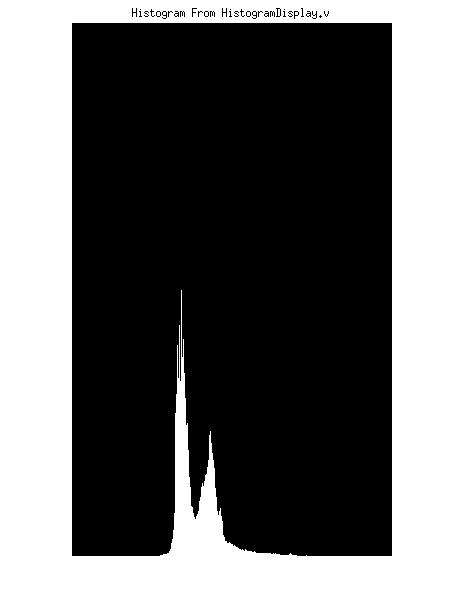
\includegraphics[scale=.8]{Images/HistogramDisplayerTestbench.png}}
    \caption{Image generated by the \texttt{Histogram Displayer module}}
    \label{fig:histogram_displayer_testbench}
  \end{figure} 
  
  \newpage
  \subsection{Total\_Module}
  In order to test \texttt{Total\_Module}, we wrote a testbench that reads in RGB values from a file, then passes those through to an instantiation of \texttt{Total\_Module} along with appropriate data valid signals. The testbench then changes the switch settings and outputs image data to file. A matlab script is used to read in this data and display images. The results are below. Clearly the module behaves correctly for the christmas shark input image, confirming our work in simulation.

\begin{table}[h!]
\begin{center}
\begin{tabular} {c c c}
  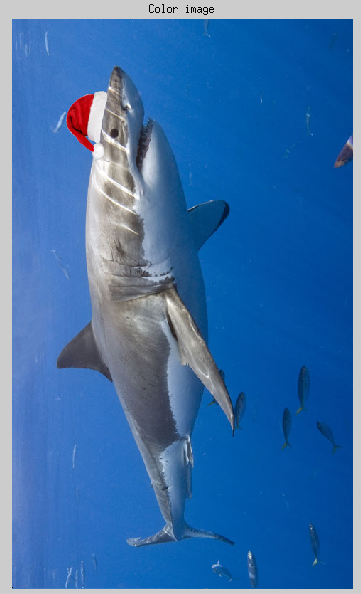
\includegraphics[scale=.52]{Images/TotalModule/RGB.png}
&
  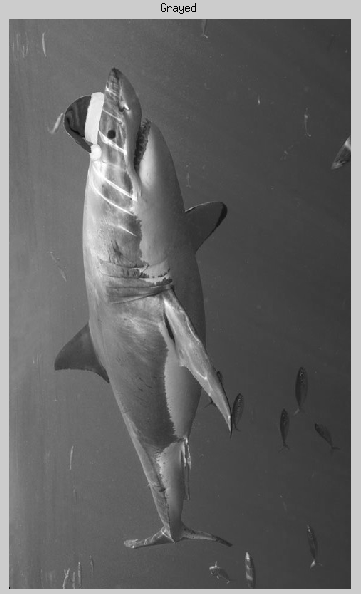
\includegraphics[scale=.52]{Images/TotalModule/Gray.png}
&
  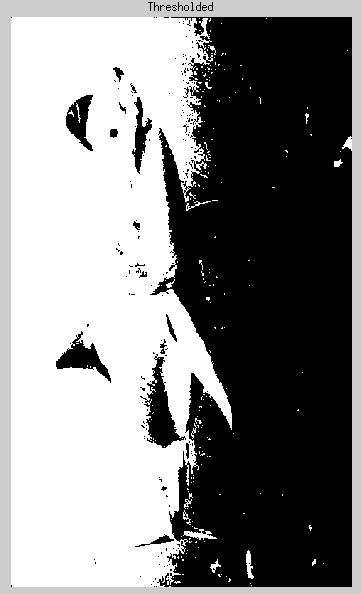
\includegraphics[scale=.52]{Images/TotalModule/Thresholded.png}
\end{tabular}
\end{center}
\captionof{figure}{RGB pass through, grayscale image, and thresholded image}
\end{table}

\begin{table}[h!]
\begin{center}
\begin{tabular} {c c}
  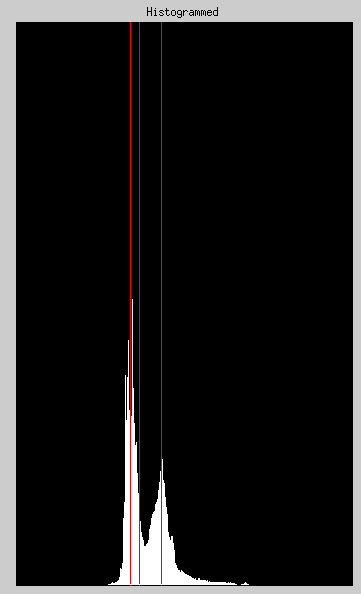
\includegraphics[scale=.8]{Images/TotalModule/Histogrammed.png}
&
  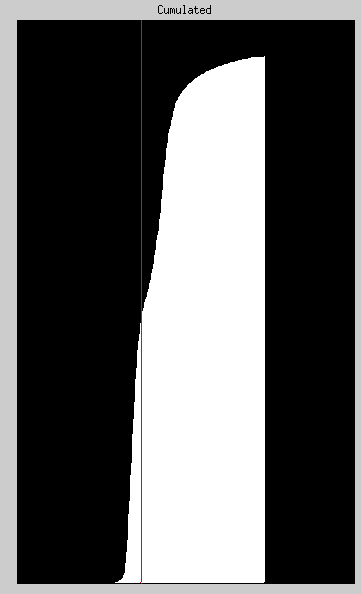
\includegraphics[scale=.8]{Images/TotalModule/Cumulated.png}
\end{tabular}
\end{center}
\captionof{figure}{Histogram and Cumulated Histogram generated by \texttt{Total\_Module}}
\end{table}
  
  \begin{table}[h!]
\begin{center}
\begin{tabular} {c c}
  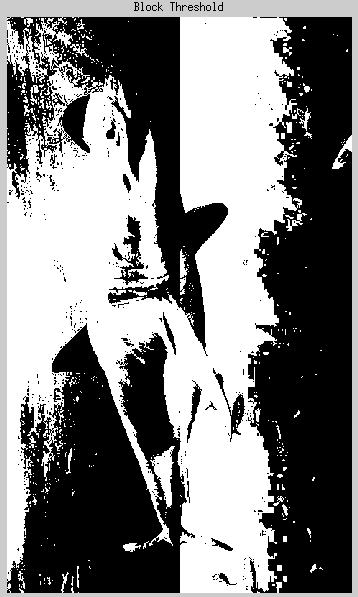
\includegraphics[scale=.8]{Images/TotalModule/BlockThresholded.png}
&
  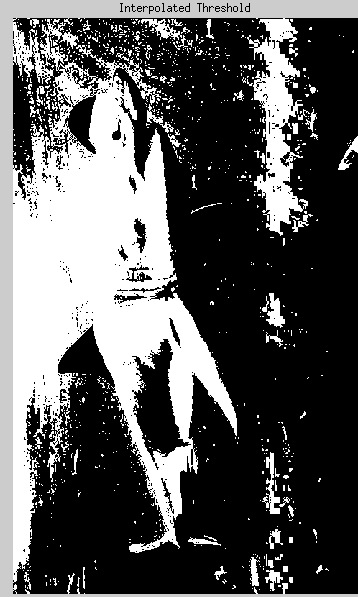
\includegraphics[scale=.8]{Images/TotalModule/SmoothThresholded.png}
\end{tabular}
\end{center}
\captionof{figure}{Histogram and Cumulated Histogram generated by \texttt{Total\_Module}}
\end{table}
  
  
  
  
\end{document}
